\documentclass[tikz,border=10pt]{standalone}
\usepackage{tikz}
\usetikzlibrary{calc}
\begin{document}
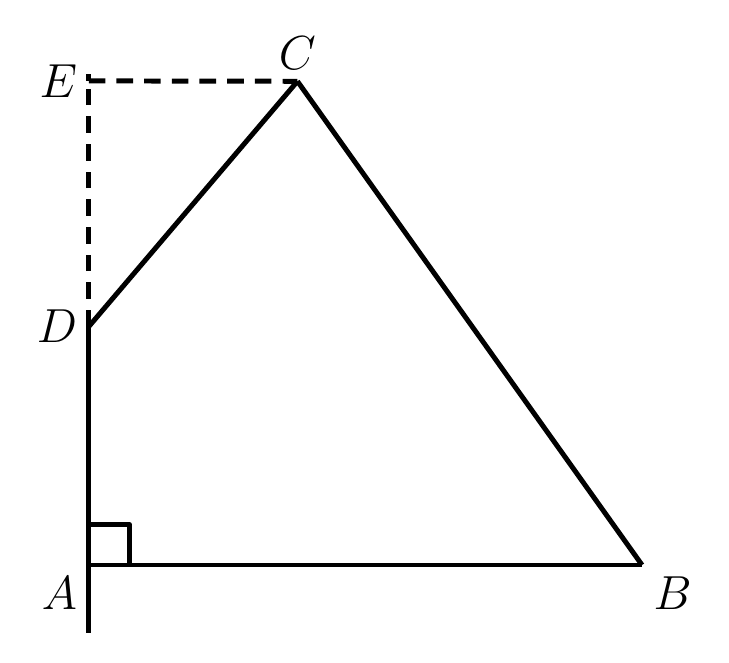
\begin{tikzpicture}[line width=1.8pt, line join=round]
  % Named coordinates (pixel -> cm, s = 0.022346, origin at A, y up)
  \coordinate (A) at (0,0);
  \coordinate (B) at (7.026,0);
  \coordinate (C) at (2.650,6.143);
  \coordinate (E) at (0,6.148);
  \coordinate (Estub) at (0,6.23);    % short dashed overhang above E
  \coordinate (D) at (0,3.028);

  % Solid segments
  \draw (A) -- (B);                    % base AB
  \draw (0,-0.86) -- (D);              % vertical A-D, slight overhang below A
  \draw (D) -- (C);                    % D-C, full length to D
  \draw (B) -- (C);                    % BC

  % Dashed segments
  \draw[dash pattern=on 6pt off 4pt] (D) -- (E);      % dashed D-E up to E
  \draw[dash pattern=on 6pt off 4pt] (E) -- (Estub);  % dashed stub past E (starts on-dash so it is visible)
  \draw[dash pattern=on 6pt off 4pt] (E) -- (C);      % horizontal E-C

  % Right-angle mark at A (only one)
  \draw (0.514,0) -- (0.514,0.514) -- (0,0.514);

  % Labels
  \node[font=\fontsize{17.5}{21}\selectfont, below left] at (A) {$A$};
  \node[font=\fontsize{17.5}{21}\selectfont, below right] at (B) {$B$};
  \node[font=\fontsize{17.5}{21}\selectfont, above] at (C) {$C$};
  \node[font=\fontsize{17.5}{21}\selectfont, left] at (E) {$E$};
  \node[font=\fontsize{17.5}{21}\selectfont, left] at (D) {$D$};
\end{tikzpicture}
\end{document}